%!TeX program = lualatex
\renewcommand{\thelektion}{L08 \textperiodcentered{} Logische Gatter I}
\usetikzlibrary{circuits.logic.US}

\begin{frame}\lessontitle{Lektion 08}{Logische Gatter I}{Vom Stromkreis zum Gatter: NOT, AND, OR \textperiodcentered{} Skript, Kapitel 4}\end{frame}

\begin{frame}\FDUtitle{Vom Stromkreis zur Information}
\begin{center}
Ein Chip ist ein Netzwerk aus leitenden Verbindungen und Schaltern.
\vspace{4mm}

\textbf{Zentrale Idee}: Elektrische Zustände werden als logische Zustände interpretiert.
\end{center}
\[
    \text{niedrige Spannung} \longleftrightarrow 0,
    \qquad
    \text{hohe Spannung} \longleftrightarrow 1.
\]
\end{frame}

\begin{frame}\FDUtitle{Warum ausgerechnet zwei Zustände?}
\begin{itemize}\setlength\itemsep{7pt}
  \item In echten Schaltungen gibt es Rauschen, Verzögerungen, Fertigungstoleranzen
  \item Man arbeitet daher mit \tib{Spannungsbereichen}, nicht mit exakten Werten
  \item Zwei klar unterscheidbare Zustände lassen sich sehr zuverlässig erkennen
\end{itemize}
\vspace{3mm}
\begin{center}
Erinnerung an Lektion 1: Shannon zeigte 1937, dass sich Boolesche Logik so elektrisch realisieren lässt.
\end{center}
\end{frame}

\begin{frame}\FDUtitle{Vom Transistor zum Gatter}
\begin{itemize}\setlength\itemsep{7pt}
  \item \tib{Transistoren} = extrem schnelle elektronische Schalter
  \item Ein logisches \tib{Gatter} ist eine konkrete Schaltung aus mehreren Transistoren
  \item Reale Gatter haben technische Kennwerte: Propagationsverzögerung, Leistungsaufnahme, Fan-out
\end{itemize}
\end{frame}

\begin{frame}\FDUtitle{Boolesche Grundverknüpfungen}
\begin{center}
Funktionen, die Bits als Eingabe erhalten und \textbf{genau ein} Bit ausgeben.
\end{center}
\vspace{4mm}
\begin{center}
\Large\bfseries\color{FDUteal}NOT \quad AND \quad OR
\end{center}
\end{frame}

\begin{frame}\FDUtitle{NOT -- Negation}
\begin{columns}[c,onlytextwidth]
\begin{column}{.46\textwidth}
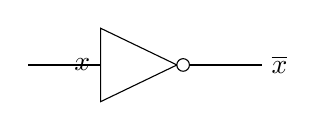
\begin{tikzpicture}[circuit logic US, scale=1.3]
  \node[not gate, draw] (not1) {};
  \draw (not1.input) ++(-0.7,0) -- (not1.input) node[left] {$x$};
  \draw (not1.output) -- ++(0.7,0) node[right] {$\overline{x}$};
\end{tikzpicture}
\end{column}
\begin{column}{.46\textwidth}
\begin{tabular}{c||c}
    $x$ & $\overline{x}$ \\\midrule\midrule
    0 & 1 \\\midrule
    1 & 0 \\
\end{tabular}
\end{column}
\end{columns}
\vspace{3mm}
\begin{center}Ein Eingang, negierter Ausgang.\end{center}
\end{frame}

\begin{frame}\FDUtitle{AND -- Konjunktion}
\begin{columns}[c,onlytextwidth]
\begin{column}{.46\textwidth}
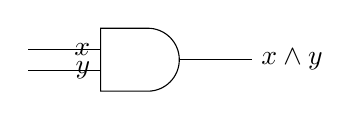
\begin{tikzpicture}[circuit logic US, scale=1.3]
  \node[and gate, draw] (and1) {};
  \draw (and1.input 1) ++(-0.7,0) -- (and1.input 1) node[left] {$x$};
  \draw (and1.input 2) ++(-0.7,0) -- (and1.input 2) node[left] {$y$};
  \draw (and1.output) -- ++(0.7,0) node[right] {$x \wedge y$};
\end{tikzpicture}
\end{column}
\begin{column}{.46\textwidth}
\begin{tabular}{c|c||c}
    $x$ & $y$ & $x \wedge y$ \\\midrule\midrule
    0 & 0 & 0 \\\midrule
    0 & 1 & 0 \\\midrule
    1 & 0 & 0 \\\midrule
    1 & 1 & 1 \\
\end{tabular}
\end{column}
\end{columns}
\vspace{3mm}
\begin{center}Ausgang 1 nur, wenn \textbf{beide} Eingänge 1 sind.\end{center}
\end{frame}

\begin{frame}\FDUtitle{OR -- Disjunktion}
\begin{columns}[c,onlytextwidth]
\begin{column}{.46\textwidth}
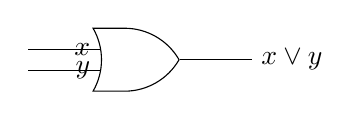
\begin{tikzpicture}[circuit logic US, scale=1.3]
  \node[or gate, draw] (or1) {};
  \draw (or1.input 1) ++(-0.7,0) -- (or1.input 1) node[left] {$x$};
  \draw (or1.input 2) ++(-0.7,0) -- (or1.input 2) node[left] {$y$};
  \draw (or1.output) -- ++(0.7,0) node[right] {$x \vee y$};
\end{tikzpicture}
\end{column}
\begin{column}{.46\textwidth}
\begin{tabular}{c|c||c}
    $x$ & $y$ & $x \vee y$ \\\midrule\midrule
    0 & 0 & 0 \\\midrule
    0 & 1 & 1 \\\midrule
    1 & 0 & 1 \\\midrule
    1 & 1 & 1 \\
\end{tabular}
\end{column}
\end{columns}
\vspace{3mm}
\begin{center}Ausgang 1, wenn \textbf{mindestens ein} Eingang 1 ist.\end{center}
\end{frame}

\begin{frame}\FDUtitle{Übung: Gatter kombinieren}
\begin{center}
Ein Fahrstuhl darf sich nur bewegen, wenn die Tür geschlossen \emph{und} entweder das Übergewicht nicht überschritten \emph{oder} der Notfall-Modus deaktiviert ist.
\vspace{4mm}

Modellieren Sie diese Bedingung mit AND-, OR- und NOT-Gattern.
\end{center}
\only<2->{\begin{center}\large $t \wedge (\overline{u} \vee \overline{n})$\end{center}}
\end{frame}

\begin{frame}{Auftrag}{Kapitel 4: Logische Grundverknüpfungen}
\aufgabebox{\textbf{Aufgabe 4.1}: Modellieren Sie die Fahrstuhl-Bedingung mithilfe von AND-, OR- und NOT-Gattern und geben Sie die logische Formel an.}
\end{frame}
